% ==================================================================

\chapter{Informatie over het vak}

\section{Puntenverdeling}

\begin{table}[H]
  \centering
  \begin{tabular}{@{}lll@{}}
    \toprule
    \textbf{Deel} & \textbf{Gewicht} & \textbf{Vorm} \\
    \midrule
    Labo & 20\,\% & Labosessies + labotest \\
    Examen hoorcollege & 80\,\% & zie hieronder \\
    \quad Theorievraag & 50\,\% van het examen & mondeling, $\geq$ 30 min voorbereiding, max.\ 10 min \\
    \quad Oefeningen & 30\,\% van het examen & schriftelijk, tussenresultaten in tabellen \\
    \quad Meerkeuzevragen & 20\,\% van het examen & schriftelijk, met giscorrectie \\
    \bottomrule
  \end{tabular}
  \caption{Puntenverdeling Elektrische Machines}
\end{table}

\TODO{verdeling labo/examen (20/80) nog bevestigen}

Het examen duurt in totaal \textbf{3 uur}. Toegelaten: niet-programmeerbare rekenmachine,
schrijfgerief, correctievloeistof. Fouten tegen voorkennis geven een niet-tolereerbaar cijfer.

\begin{table}[H]
  \centering
  \begin{tabular}{@{}ll@{}}
    \toprule
    \textbf{Cijfer} & \textbf{Wat je moet kunnen} \\
    \midrule
    Tolereerbaar & Werking, karakteristieken en schema's reproduceren \\
    Credit & Ze ook verklaren \\
    Onderscheiding & Redeneren en elementen combineren met inzicht \\
    \bottomrule
  \end{tabular}
\end{table}

\section{Giscorrectie meerkeuze}

\begin{table}[H]
  \centering
  \begin{tabular}{@{}lll@{}}
    \toprule
    \textbf{Aangeduid} & \textbf{Juiste erbij} & \textbf{Juiste niet erbij} \\
    \midrule
    1 & $+1$ & $-1/3$ \\
    2 & $+1/3$ & $-1/3$ \\
    3 & $+1/9$ & $-1/3$ \\
    0 of 4 & $0$ & $0$ \\
    \bottomrule
  \end{tabular}
\end{table}

Aanpassen: vakje wegwissen met correctievloeistof, \textbf{niet} opnieuw tekenen.


\section{Handboeken}
Chapman, "Electric machinery fundamentals", McGraw-Hill, 2012. ISBN: 9780071325813 

\section{InhoudsTabel}

\begin{figure}[H]
  \centering
  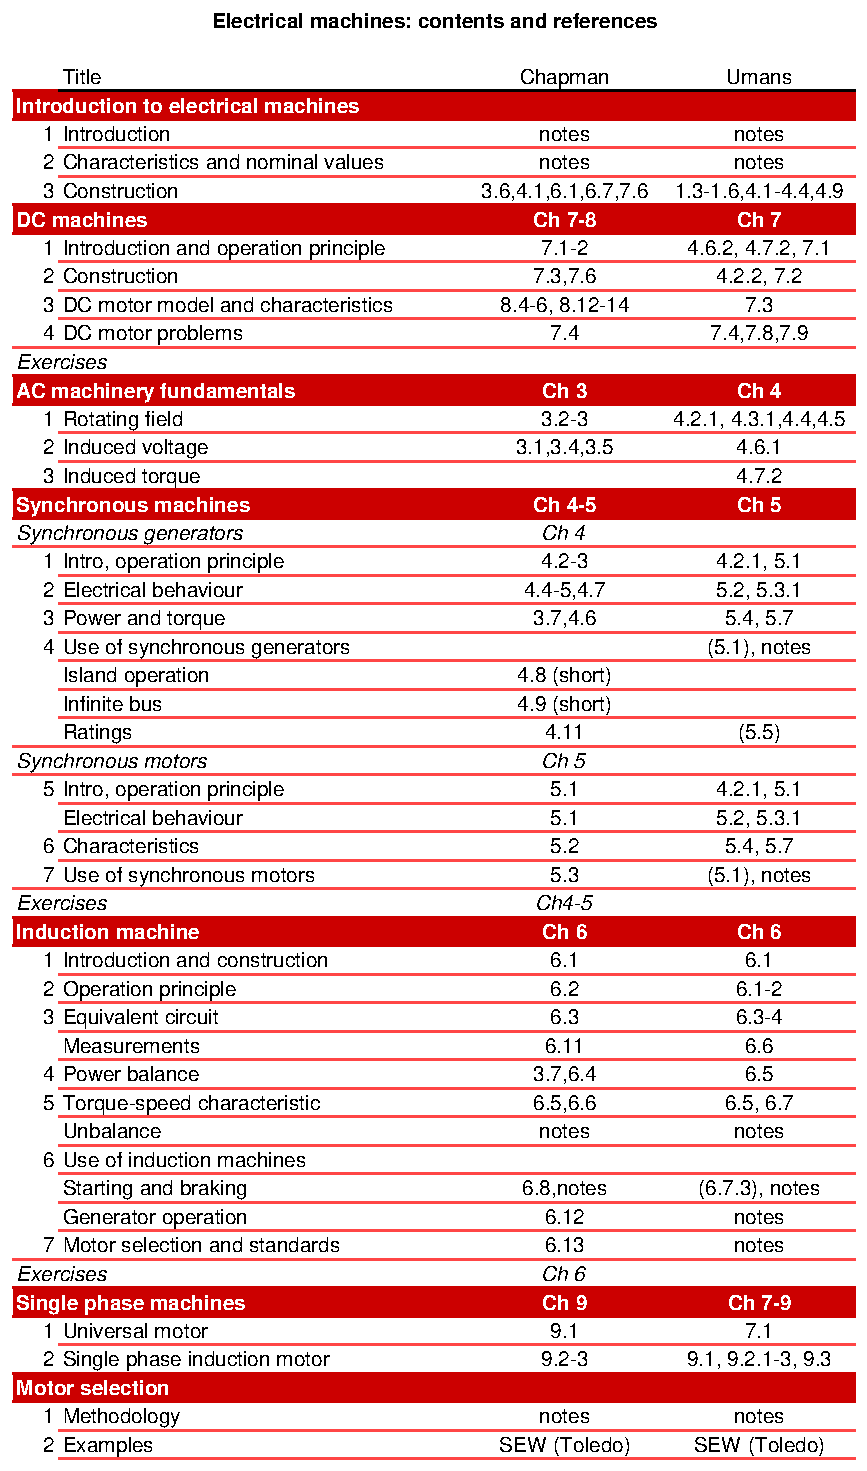
\includegraphics[width=\textwidth,height=0.85\textheight,keepaspectratio]{assets/inhoudstafel.pdf}
  \caption{Inhoudstafel van de cursus met verwijzingen naar Chapman en Umans}
  \label{fig:inhoudstafel}
\end{figure}

\newpage

